
%% bare_jrnl_compsoc.tex
%% V1.4a
%% 2014/09/17
%% by Michael Shell
%% See:
%% http://www.michaelshell.org/
%% for current contact information.
%%
%% This is a skeleton file demonstrating the use of IEEEtran.cls
%% (requires IEEEtran.cls version 1.8a or later) with an IEEE
%% Computer Society journal paper.
%%
%% Support sites:
%% http://www.michaelshell.org/tex/ieeetran/
%% http://www.ctan.org/tex-archive/macros/latex/contrib/IEEEtran/
%% and
%% http://www.ieee.org/

%%*************************************************************************
%% Legal Notice:
%% This code is offered as-is without any warranty either expressed or
%% implied; without even the implied warranty of MERCHANTABILITY or
%% FITNESS FOR A PARTICULAR PURPOSE! 
%% User assumes all risk.
%% In no event shall IEEE or any contributor to this code be liable for
%% any damages or losses, including, but not limited to, incidental,
%% consequential, or any other damages, resulting from the use or misuse
%% of any information contained here.
%%
%% All comments are the opinions of their respective authors and are not
%% necessarily endorsed by the IEEE.
%%
%% This work is distributed under the LaTeX Project Public License (LPPL)
%% ( http://www.latex-project.org/ ) version 1.3, and may be freely used,
%% distributed and modified. A copy of the LPPL, version 1.3, is included
%% in the base LaTeX documentation of all distributions of LaTeX released
%% 2003/12/01 or later.
%% Retain all contribution notices and credits.
%% ** Modified files should be clearly indicated as such, including  **
%% ** renaming them and changing author support contact information. **
%%
%% File list of work: IEEEtran.cls, IEEEtran_HOWTO.pdf, bare_adv.tex,
%%                    bare_conf.tex, bare_jrnl.tex, bare_conf_compsoc.tex,
%%                    bare_jrnl_compsoc.tex, bare_jrnl_transmag.tex
%%*************************************************************************


% *** Authors should verify (and, if needed, correct) their LaTeX system  ***
% *** with the testflow diagnostic prior to trusting their LaTeX platform ***
% *** with production work. IEEE's font choices and paper sizes can       ***
% *** trigger bugs that do not appear when using other class files.       ***                          ***
% The testflow support page is at:
% http://www.michaelshell.org/tex/testflow/


\documentclass[10pt,conference,onecolumn,compsoc]{IEEEtran}


\usepackage{hyperref}
\usepackage{enumitem}
\setlist[itemize]{leftmargin=3 cm}
\setlist[enumerate]{leftmargin=3cm}



% *** CITATION PACKAGES ***
%
\ifCLASSOPTIONcompsoc
  % IEEE Computer Society needs nocompress option
  % requires cite.sty v4.0 or later (November 2003)
  \usepackage[nocompress]{cite}
\else
  % normal IEEE
  \usepackage{cite}
\fi
% cite.sty was written by Donald Arseneau
% V1.6 and later of IEEEtran pre-defines the format of the cite.sty package
% \cite{} output to follow that of IEEE. Loading the cite package will
% result in citation numbers being automatically sorted and properly
% "compressed/ranged". e.g., [1], [9], [2], [7], [5], [6] without using
% cite.sty will become [1], [2], [5]--[7], [9] using cite.sty. cite.sty's
% \cite will automatically add leading space, if needed. Use cite.sty's
% noadjust option (cite.sty V3.8 and later) if you want to turn this off
% such as if a citation ever needs to be enclosed in parenthesis.
% cite.sty is already installed on most LaTeX systems. Be sure and use
% version 5.0 (2009-03-20) and later if using hyperref.sty.
% The latest version can be obtained at:
% http://www.ctan.org/tex-archive/macros/latex/contrib/cite/
% The documentation is contained in the cite.sty file itself.



% *** GRAPHICS RELATED PACKAGES ***
%
\ifCLASSINFOpdf
   \usepackage[pdftex]{graphicx}
 
\else
 
\fi
% graphicx was written by David Carlisle and Sebastian Rahtz. It is
% required if you want graphics, photos, etc. graphicx.sty is already
% installed on most LaTeX systems. The latest version and documentation
% can be obtained at: 
% http://www.ctan.org/tex-archive/macros/latex/required/graphics/
% Another good source of documentation is "Using Imported Graphics in
% LaTeX2e" by Keith Reckdahl which can be found at:
% http://www.ctan.org/tex-archive/info/epslatex/
%
% latex, and pdflatex in dvi mode, support graphics in encapsulated
% postscript (.eps) format. pdflatex in pdf mode supports graphics
% in .pdf, .jpeg, .png and .mps (metapost) formats. Users should ensure
% that all non-photo figures use a vector format (.eps, .pdf, .mps) and
% not a bitmapped formats (.jpeg, .png). IEEE frowns on bitmapped formats
% which can result in "jaggedy"/blurry rendering of lines and letters as
% well as large increases in file sizes.
%
% You can find documentation about the pdfTeX application at:
% http://www.tug.org/applications/pdftex









% *** PDF, URL AND HYPERLINK PACKAGES ***
%
\usepackage{url}
% url.sty was written by Donald Arseneau. It provides better support for
% handling and breaking URLs. url.sty is already installed on most LaTeX
% systems. The latest version and documentation can be obtained at:
% http://www.ctan.org/tex-archive/macros/latex/contrib/url/
% Basically, \url{my_url_here}.




\begin{document}

\title{3ly-Zium\\ for UTM CSCI 352}
%
%

% received ..."  text while in non-compsoc journals this is reversed. Sigh.

\author{Colin Weatherly, Blade Johnson% <-this % stops a space
}

\IEEEtitleabstractindextext{%
\begin{abstract}
The project is a video game in the 2D platformer genre. The player is made to run through a level, and upon each successful completion, the level is changed to increase the difficulty. The intended target is people that play video games, primarily those that stream games as live reactions mesh well with high difficulties.
\end{abstract}

}


% make the title area
\maketitle



\IEEEdisplaynontitleabstractindextext

\IEEEpeerreviewmaketitle



\section{Introduction}



This project is a video game in the genre of 2D platformer. The goal of the game is to reach the exit of the level that the player character is placed in. The level’s layout will progressively get more complex with each clear, along with adding new hazards that increase the difficulty further. The penalty for failing a level is to be sent back to the beginning of said level, allowing the player to learn the level with every attempt.

The targeted audience for this project is people in the 18-34 age group who play video games on a regular basis. Specifically, those in the age group that livestream games. Due to the increasingly difficult challenge that the game provides, having live reactions of attempts to beat the game will provide content for the targeted audience.



\subsection{Background}
A 2D platformer is a game genre set on a 2D plane where the player controlled character must move and jump to avoid obstacles and reach the end.

We decided to make a platforming game because of our love for games in general and our shared interest in platformers. Because of this, we feel we can properly create one.

% needed in second column of first page if using \IEEEpubid
%\IEEEpubidadjcol


\subsection{Impacts}
This project is not meant to impact the world in some way. The point of a game is to provide entertainment, which will only impact a portion of the population if it were to gain traction within the community. At the current time, there is no plan for a meaningful story in the game, so the impact will be purely driven by the quality of the gameplay.

\subsection{Challenges}
The main challenges will most likely be coding the physics of the player character; developing new mechanics instead of being purely moving and jumping; keeping the game fun despite the difficulty.


\section{Scope}
This platforming game is considered done once three levels of the game are playable from start to finish with minimal bugs or exploits. The player should be able to get through these stages without too much unnecessary frustration with either the difficulty of these stages or the control of the player character. The player character should be fully implemented with all moves intact (moving, jumping) and all hazards(such as spikes) should fail the level upon contact with the player character. As a stretch goal, we want to include more levels with new hazards. An additional stretch goal is the addition of extra moves(i.e walljumping, sliding) the player character requires to progress in more difficult levels. An additional stretch goal is scaling the window and the game assets to fit more than one resolution.

\subsection{Requirements}

\subsubsection{Functional}
\begin{itemize}
\item User inputs via designated keys are read – the application should register the inputs and move the player character accordingly
\item Selecting Start places the user in the first level – Unlike the level select which allows the user to choose a level, pressing the start button will immediately bring them to the first level
\item Level fails upon contact with a hazard – should the player character run into a hazard(i.e spike), level is failed and character is returned to the starting point of the same level
\end{itemize}

\subsubsection{Non-Functional}
\begin{itemize}
\item The game correctly displays in a 1280x720 resolution window
\item The game runs at a smooth framerate, preferably 30 frames per second
\item User's inputs have little to no delay, preferably under half a second
\end{itemize}

\subsection{Use Cases}
These are cases in which the user will interact with the program's user interface. The use cases can be seen in Table \ref{tab:useCaseIndex}.




\begin{table}
\centering
\begin{tabular}{|c|c|c|c|c|}
\hline
Use Case ID & Use Case Name & Primary Actor & Complexity & Priority \\
\hline \hline
1 & Start New Game & User & Low & 1\\
\hline
2 & Level Select & User & Low & 1\\
\hline
3 & Character Jump & User & Medium & 1\\
\hline
4 & Character Dash & User & Medium & 1\\

\end{tabular}
\caption{Use case table}
\label{tab:useCaseIndex}
\end{table}


\begin{itemize}
\item[Use Case Number:] 1
\item[Use Case Name:] Start New Game
\item[Description:] The player decides to begin the game from the beginning (Level 1). They will click on the ``Start" button (see Figure \ref{Start Mockup}). This will load the first level of the game (see Figure \ref{Level1 Mockup}).
\end{itemize}

Process flow:

\begin{enumerate}
\item Player starts the program, which begins with the main menu loaded.
\item The player left-clicks the ``Start" option on the menu.
\item The game state is updated to gameplay, and the first level is loaded.
\item[Termination Outcome:] Gameplay has begun in level 1.
\end{enumerate}

\begin{itemize}
\item[Use Case Number:] 2
\item[Use Case Name:] Level Select
\item[Description:] The player is on the main menu. The player wishes to choose a specific level in the game to play. They will left-click the ``Level Select" button on the main menu, and the screen will update to show a list of levels in vertical descending order. The player then left-click a button corresponding to a specific level, and the game will load the corresponding level (see Figure \ref{Select Mockup}).
\end{itemize}

Process flow:

\begin{enumerate}
\item Player starts the program, which begins with the main menu loaded.
\item The player left-clicks the ``Level Select" option on the main menu.
\item The level select screen is loaded, showing each level vertically in numerically descending order.
\item The player left-clicks the option corresponding to their desired level.
\item The game state is updated to gameplay, and the corresponding level loads.
\item[Termination Outcome:] Gameplay has begun in the player's selected level.
\end{enumerate}

\begin{itemize}
\item[Use Case Number:] 3
\item[Use Case Name:] Character Jump
\item[Description:] The player is in gameplay. They wish to make the player character jump (in order to avoid hazards such as spikes). The player then hits the 'Z' key. The player character will then leap upward. The character will gradually rise up off the ground for a few seconds, then gradually fall back to the ground.
\end{itemize}

Process flow:

\begin{enumerate}
\item Player is in a stage of gameplay.
\item The player presses the 'Z' key.
\item The player character then leaps off the ground into the air.
\item After a few seconds of gradually rising upward, the player character then gradually falls until hitting the ground.
\item[Termination Outcome:] The player character has completed a full jump.
\end{enumerate}

\begin{itemize}
\item[Use Case Number:] 4
\item[Use Case Name:] Character Dash
\item[Description:] The player is in gameplay. They wish to make a character quickly travel horizontally. The player then hits the 'X' key. The player will then gain a burst of speed in the direction they are moving. This can also be used during a jump.
\end{itemize}

Process flow:

\begin{enumerate}
\item Player is in a stage of gameplay.
\item The player presses the 'X' key.
\item The player's movement speed is doubled in the direction of movement(left, right) for a second.
\item[Termination Outcome:] The player has completed a full dash.
\end{enumerate}


\subsection{Interface Mockups}
\begin{figure}[ht!]
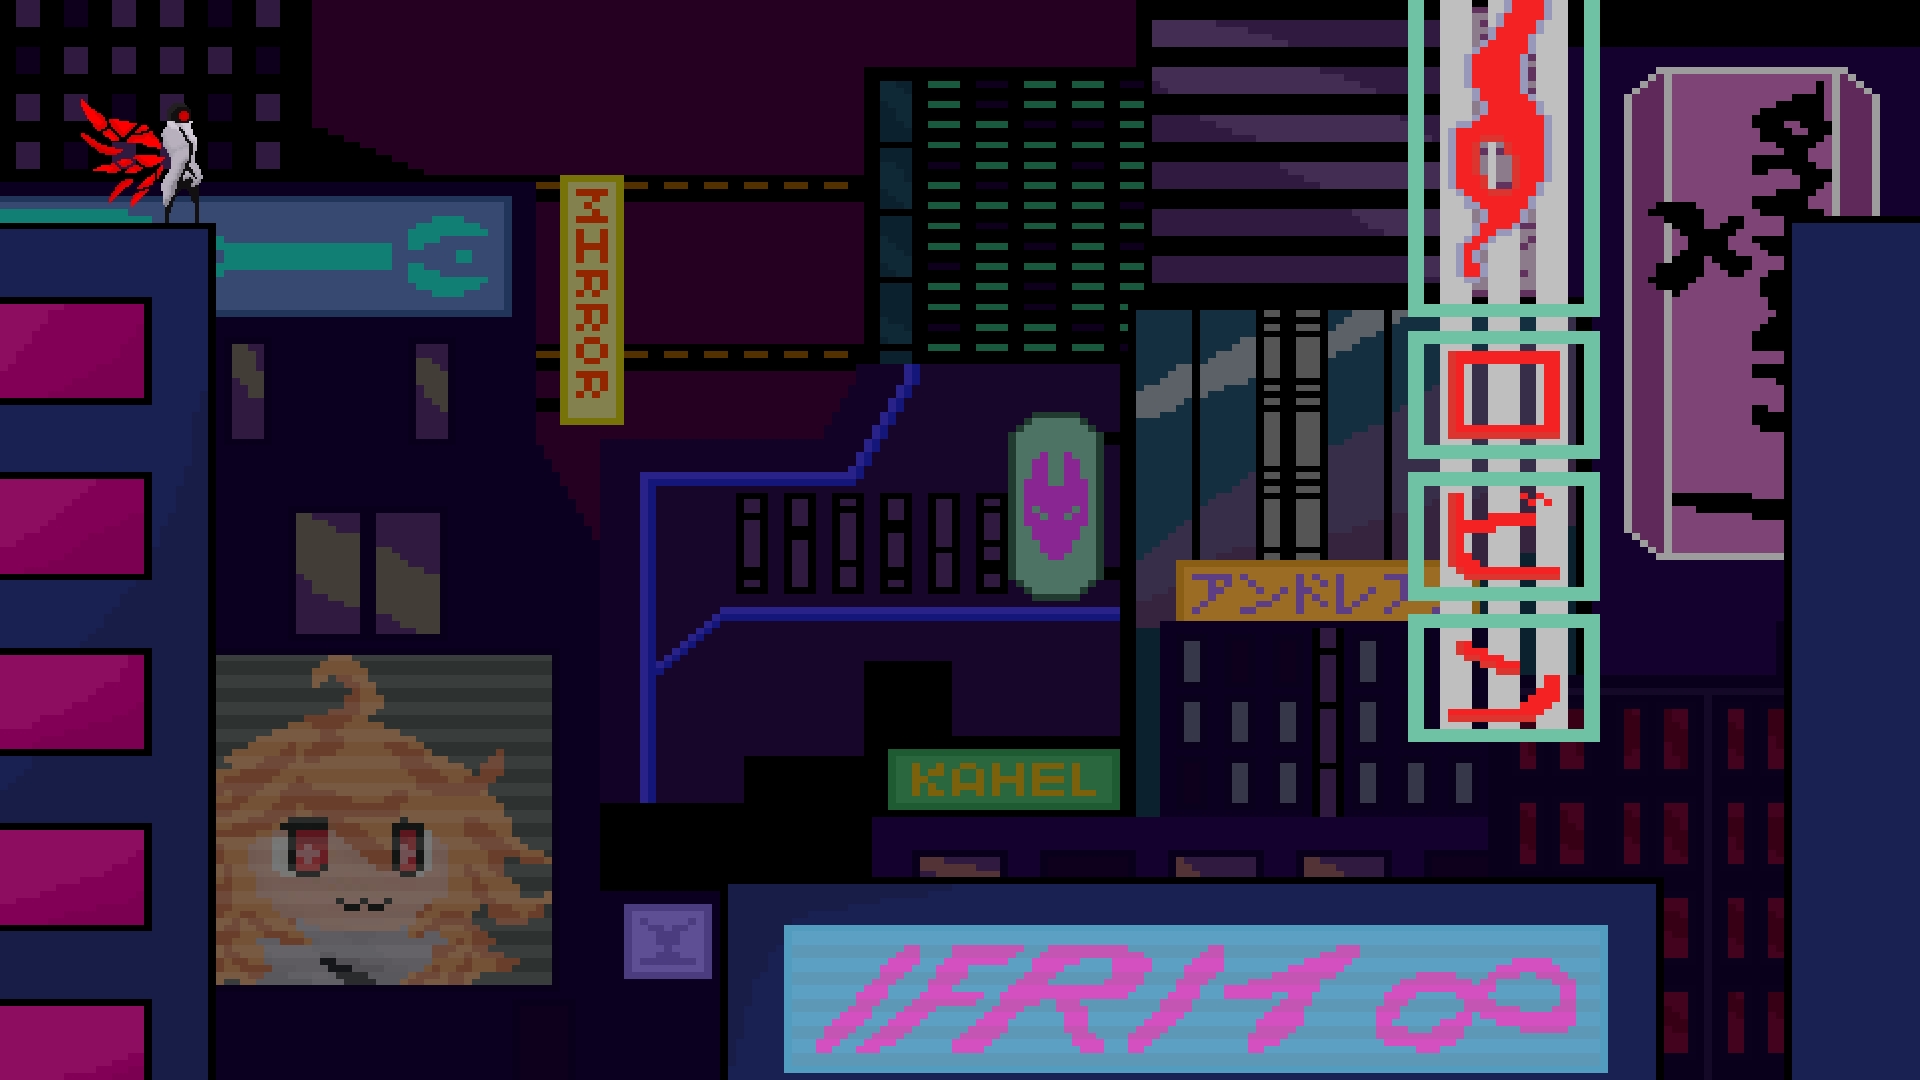
\includegraphics[height=250px, width=400px]{Level1 Mockup.png}
\caption{Mockup of a player loading into level 1}
\label{Level1 Mockup}
\end{figure}

\begin{figure}[ht!]
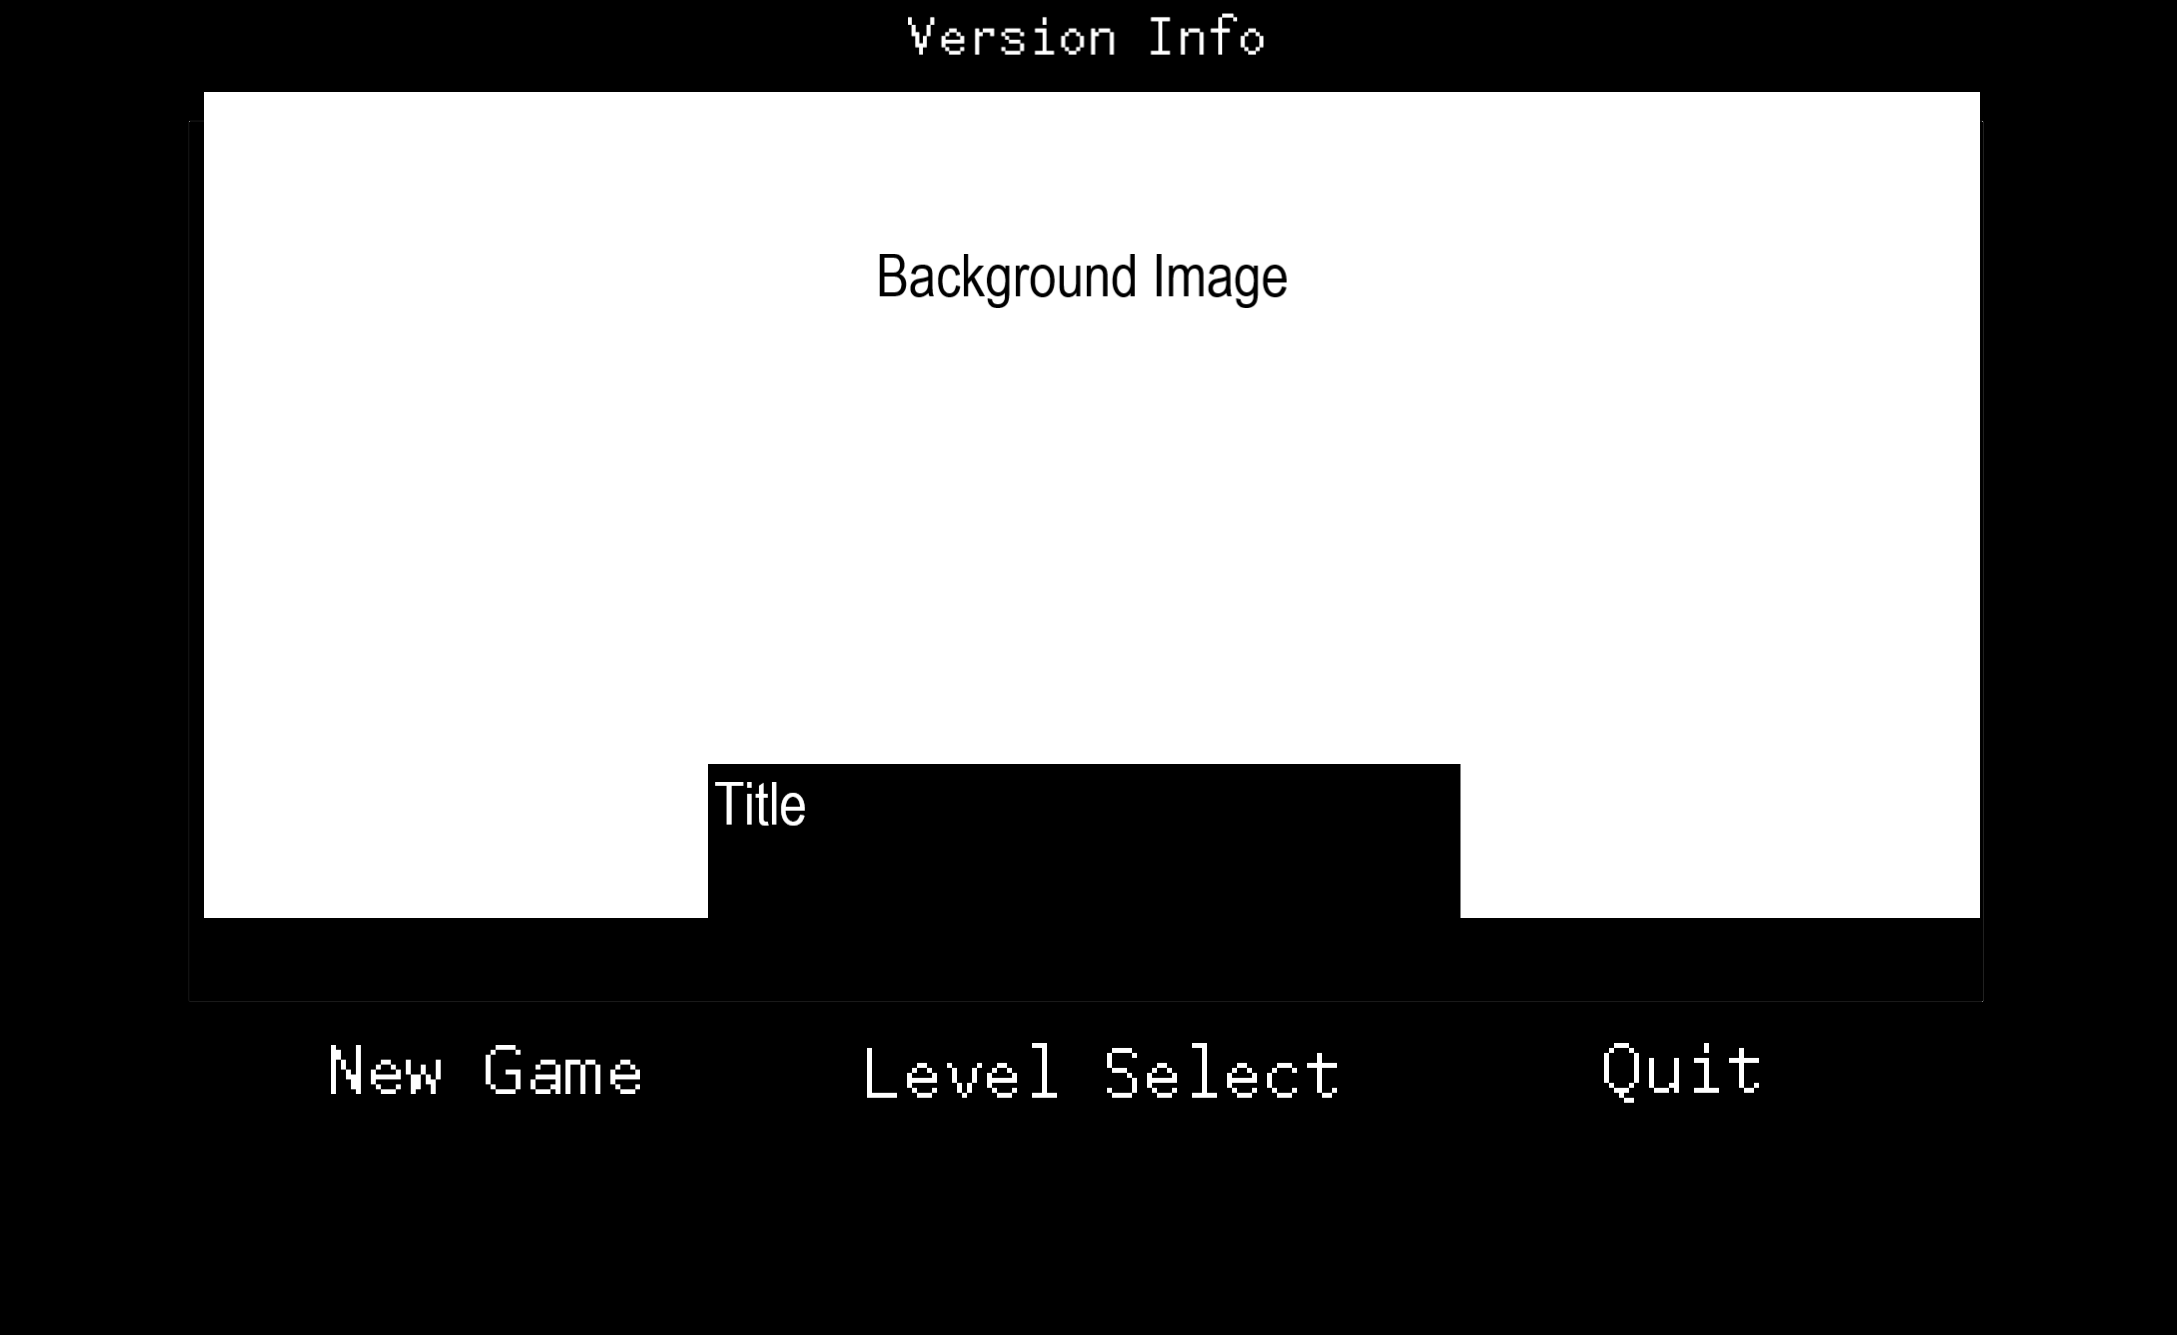
\includegraphics[height=250px, width=400px]{Start Mockup.png}
\caption{Mockup of the main menu screen}
\label{Start Mockup}
\end{figure}

\begin{figure}[ht!]
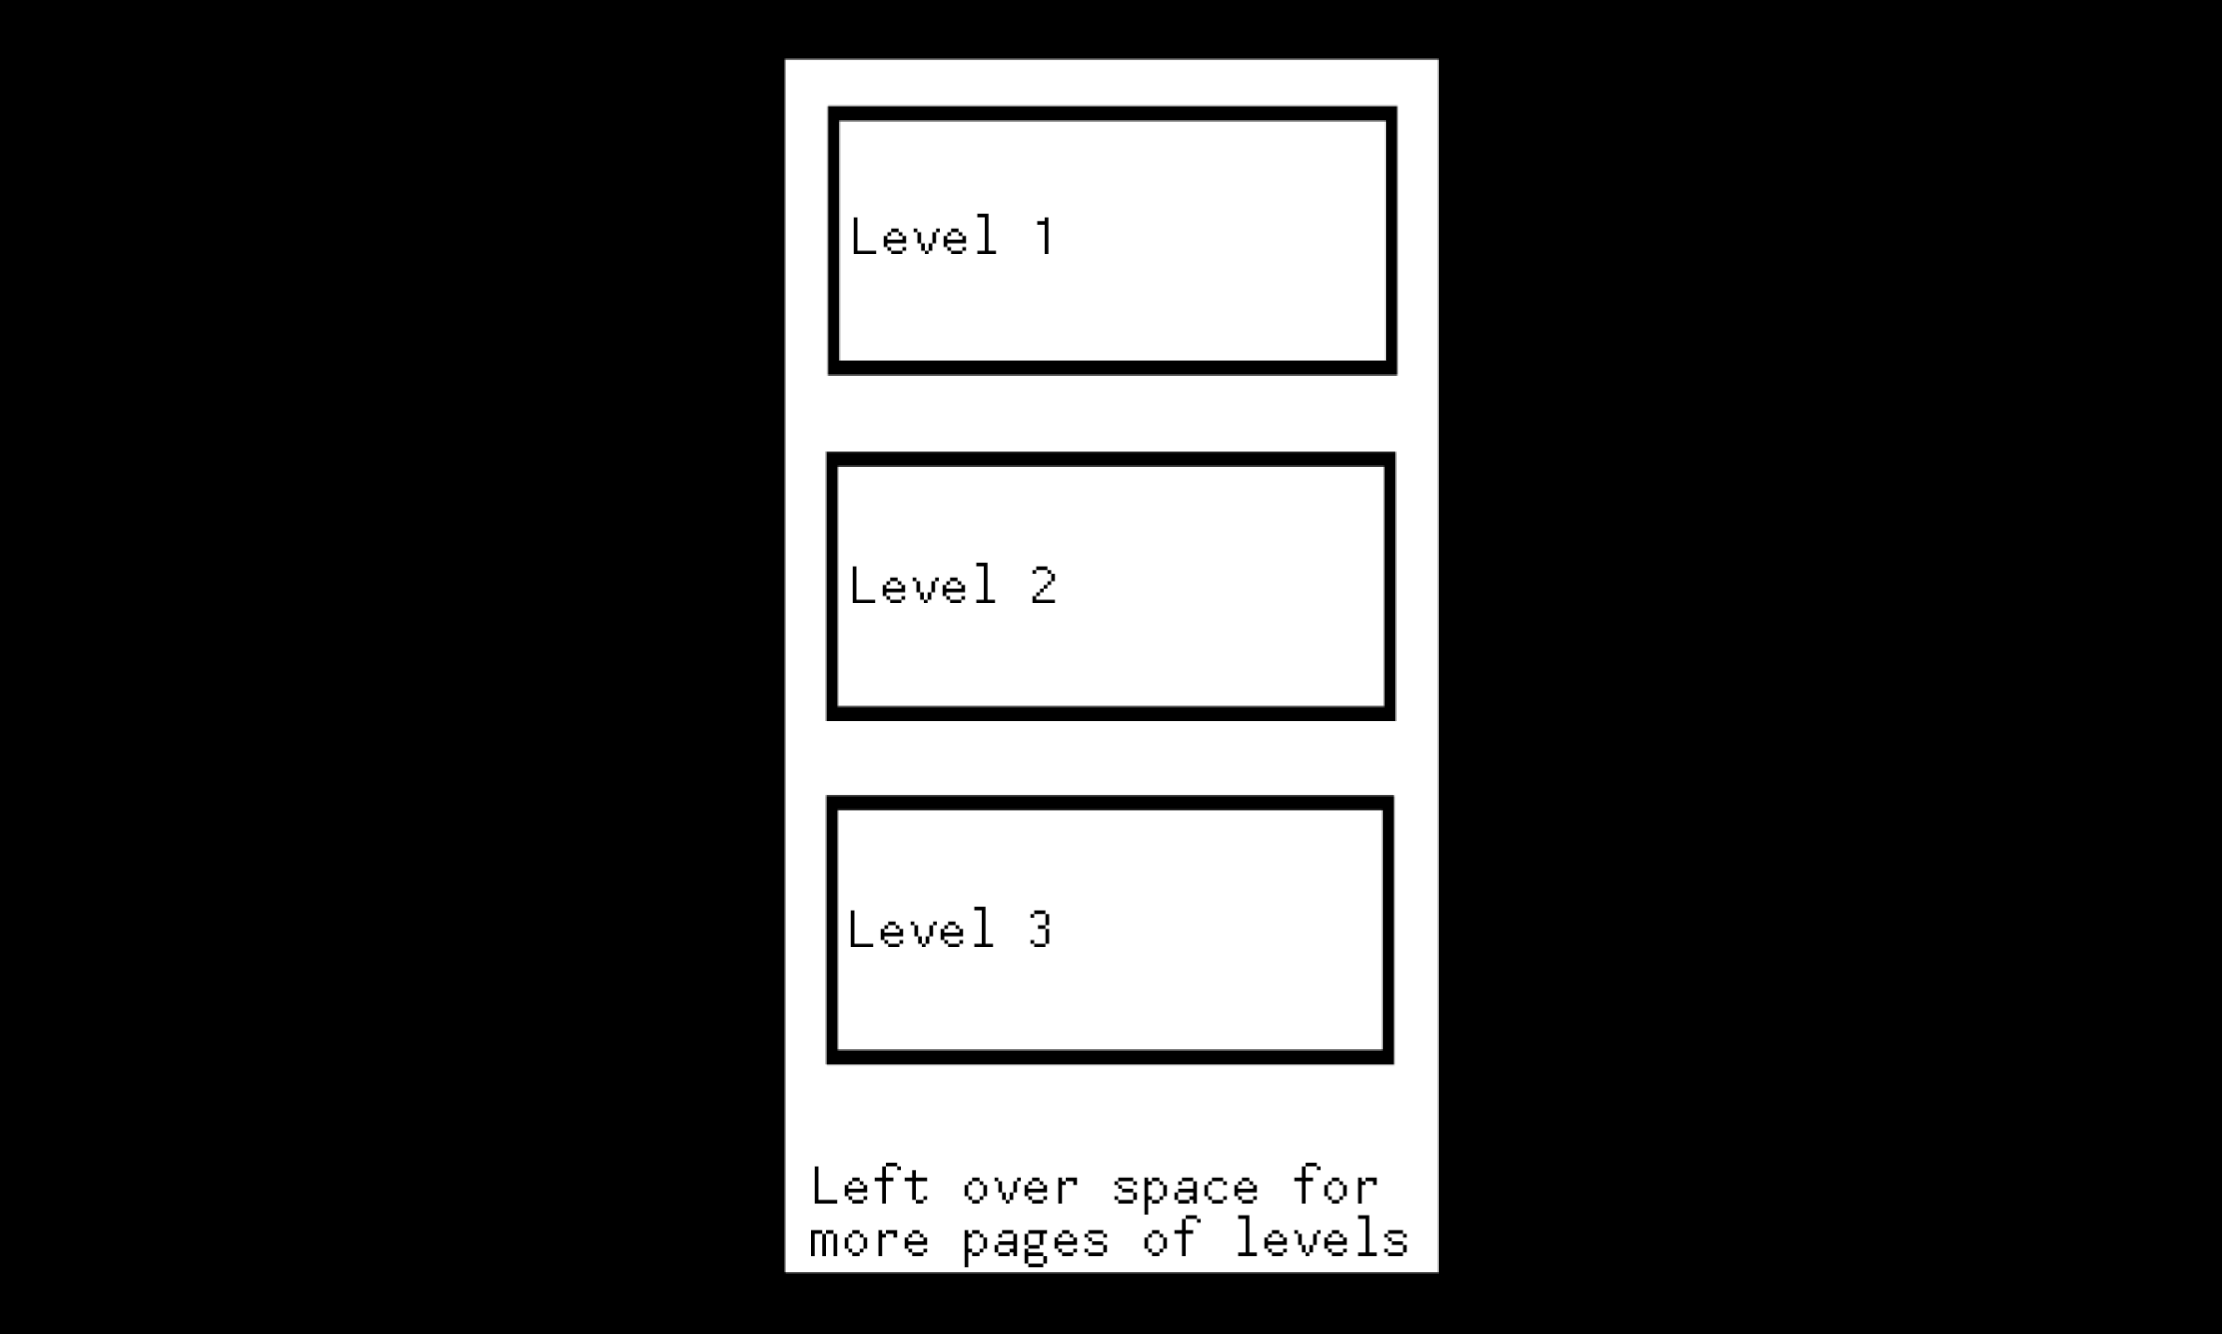
\includegraphics[height=250px, width=400px]{Select Mockup.png}
\caption{Mockup of the level select screen}
\label{Select Mockup}
\end{figure}



\section{Project Timeline}
Refer to Figure \ref{Timeline}.

The first item is where we propose the idea of a 2D platformer game.

The second item sees us writing up use cases and setting requirements. Concepts are put into place with mockups being created.

The third item is where the project is updated with designs that are more fleshed out and close to final. Initial structure ideas are outlined in a preliminary UML.

The fourth item has movement being more or less completed, with wall and ground collision now being worked on.

The fifth item has collision being finished or nearly finished. Level loading has begun implementation or is approaching implementation.

The sixth item has level loading finished or nearing completion. Menus have begun implementation. Bug testing has begun.

The last item has the project being completed, having met all goals and running with few bugs.
\begin{figure}[ht!]
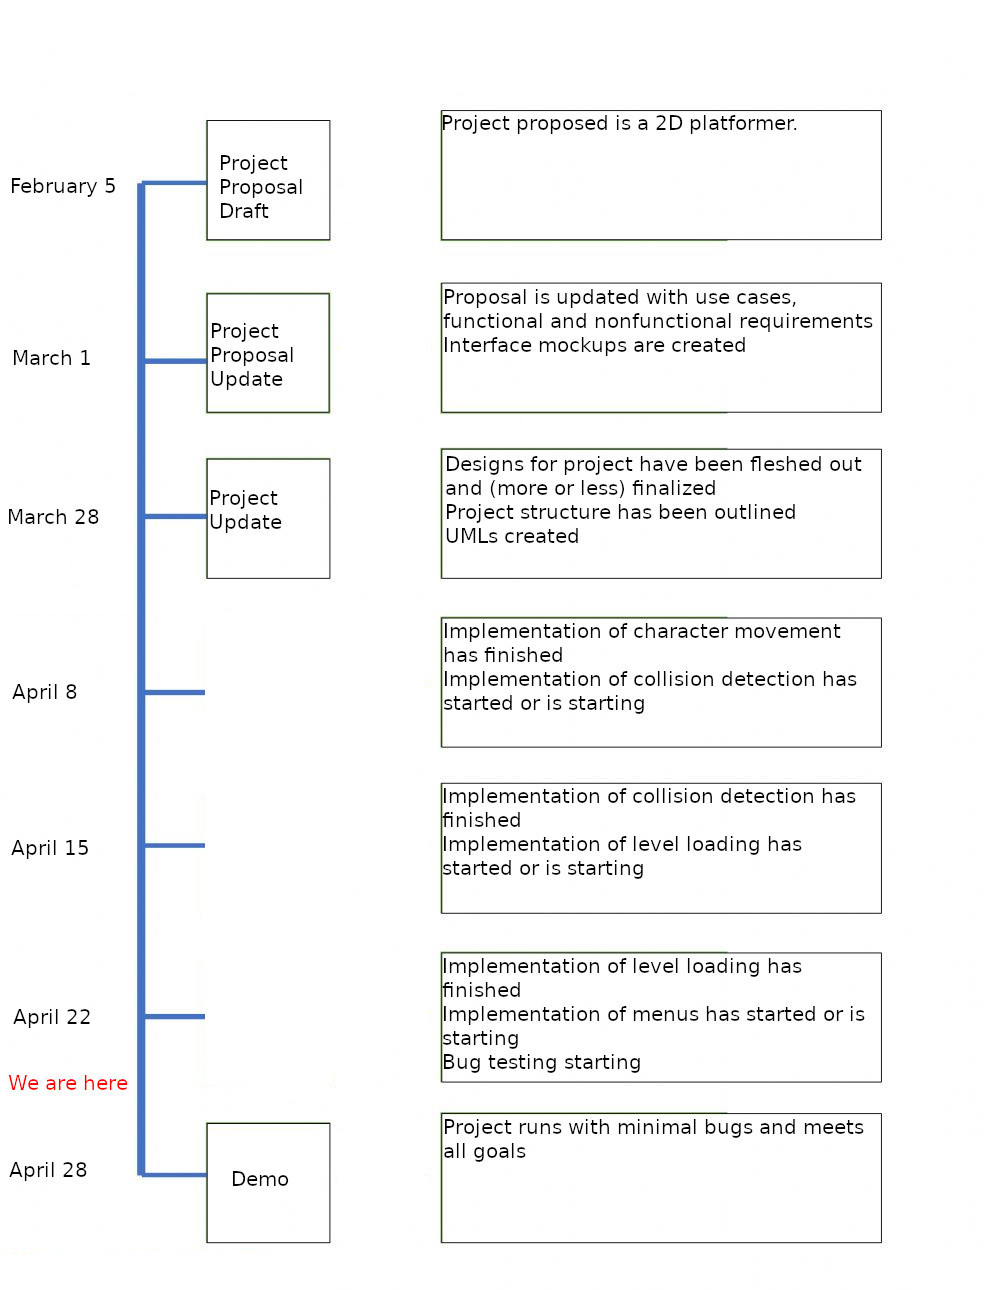
\includegraphics[height=400px, width=300px]{Timeline.jpg}
\caption{Timeline}
\label{Timeline}
\end{figure}


\section{Project Structure}
From main, the menus will be loaded. From here, StartMenu will contain methods for all of the choices, which will start the game, access the LevelSelect, or close the program. The LevelSelect and StartMenu can both load into the gameplay. Game runs the gameplay. From here, collision is loaded for the stage from a Collision object, which is a child of the Load class, which handles the loading of the correct stage. The Character is also loaded, which contains all of the information of the character, including the character’s position and collision. The movement classes helps with Character movement handling, such as jumping, horizontal movement, and jumping collision.

\subsection{UML Outline}
Refer to Figure \ref{Facade}.

Title is what the user loads into upon start up. LoadLevelSelect() creates an instance of LevelSelect, and StartGame loads an instance of Level1. CloseGame() simply closes the program.

LevelSelect is where the user can select any of the 3 levels. LoadLevel1() creates an instance of Level1, LoadLevel2() creates an instance of Level2, LoadLevel3() creates an instance of Level3, and GoBack() goes back to Title.

Each of the Level child classes contains a Player object (the object the user controls), a List of Surface objects (the walls/grounds in the stage), and a Goal object. These vary depending on the level.
The Player object inherits from the RectangleAdapter. It contains a Rectangle, is DispatcherTimer, and booleans for player movement. The object is created with x and y coordinates, which determine where the object spawns on the screen. The keyisdown and keyisup function handles movement when pressing down and releasing the arrow keys or action keys. The dtClockTime\_Tick function refreshes the object's state every few frames.

The Surface object and Goal object are both children of the Collision interface and also inherit from RectangleAdapter. Both contain a hitbox Rectangle, a Player object, and contain a DispatchTimer. Both take a Rectangle and Player object as arguments. The Goal object contains a bool that represents if it is or isn't making contact with the Player object. dtClockTime\_Tick in the Surface class handles collision between it and the player every timer tick. The Goal class checks to see if the Player has made contact with the object. If it has, the bool is set to true.

The RectangleAdapter class adapts a Rectangle into a RectangleAdapter type, which allows Surface, Goal, and Player objects to inherit from it. This is to get around the Rectangle class being a sealed class.
\begin{figure}[ht!]
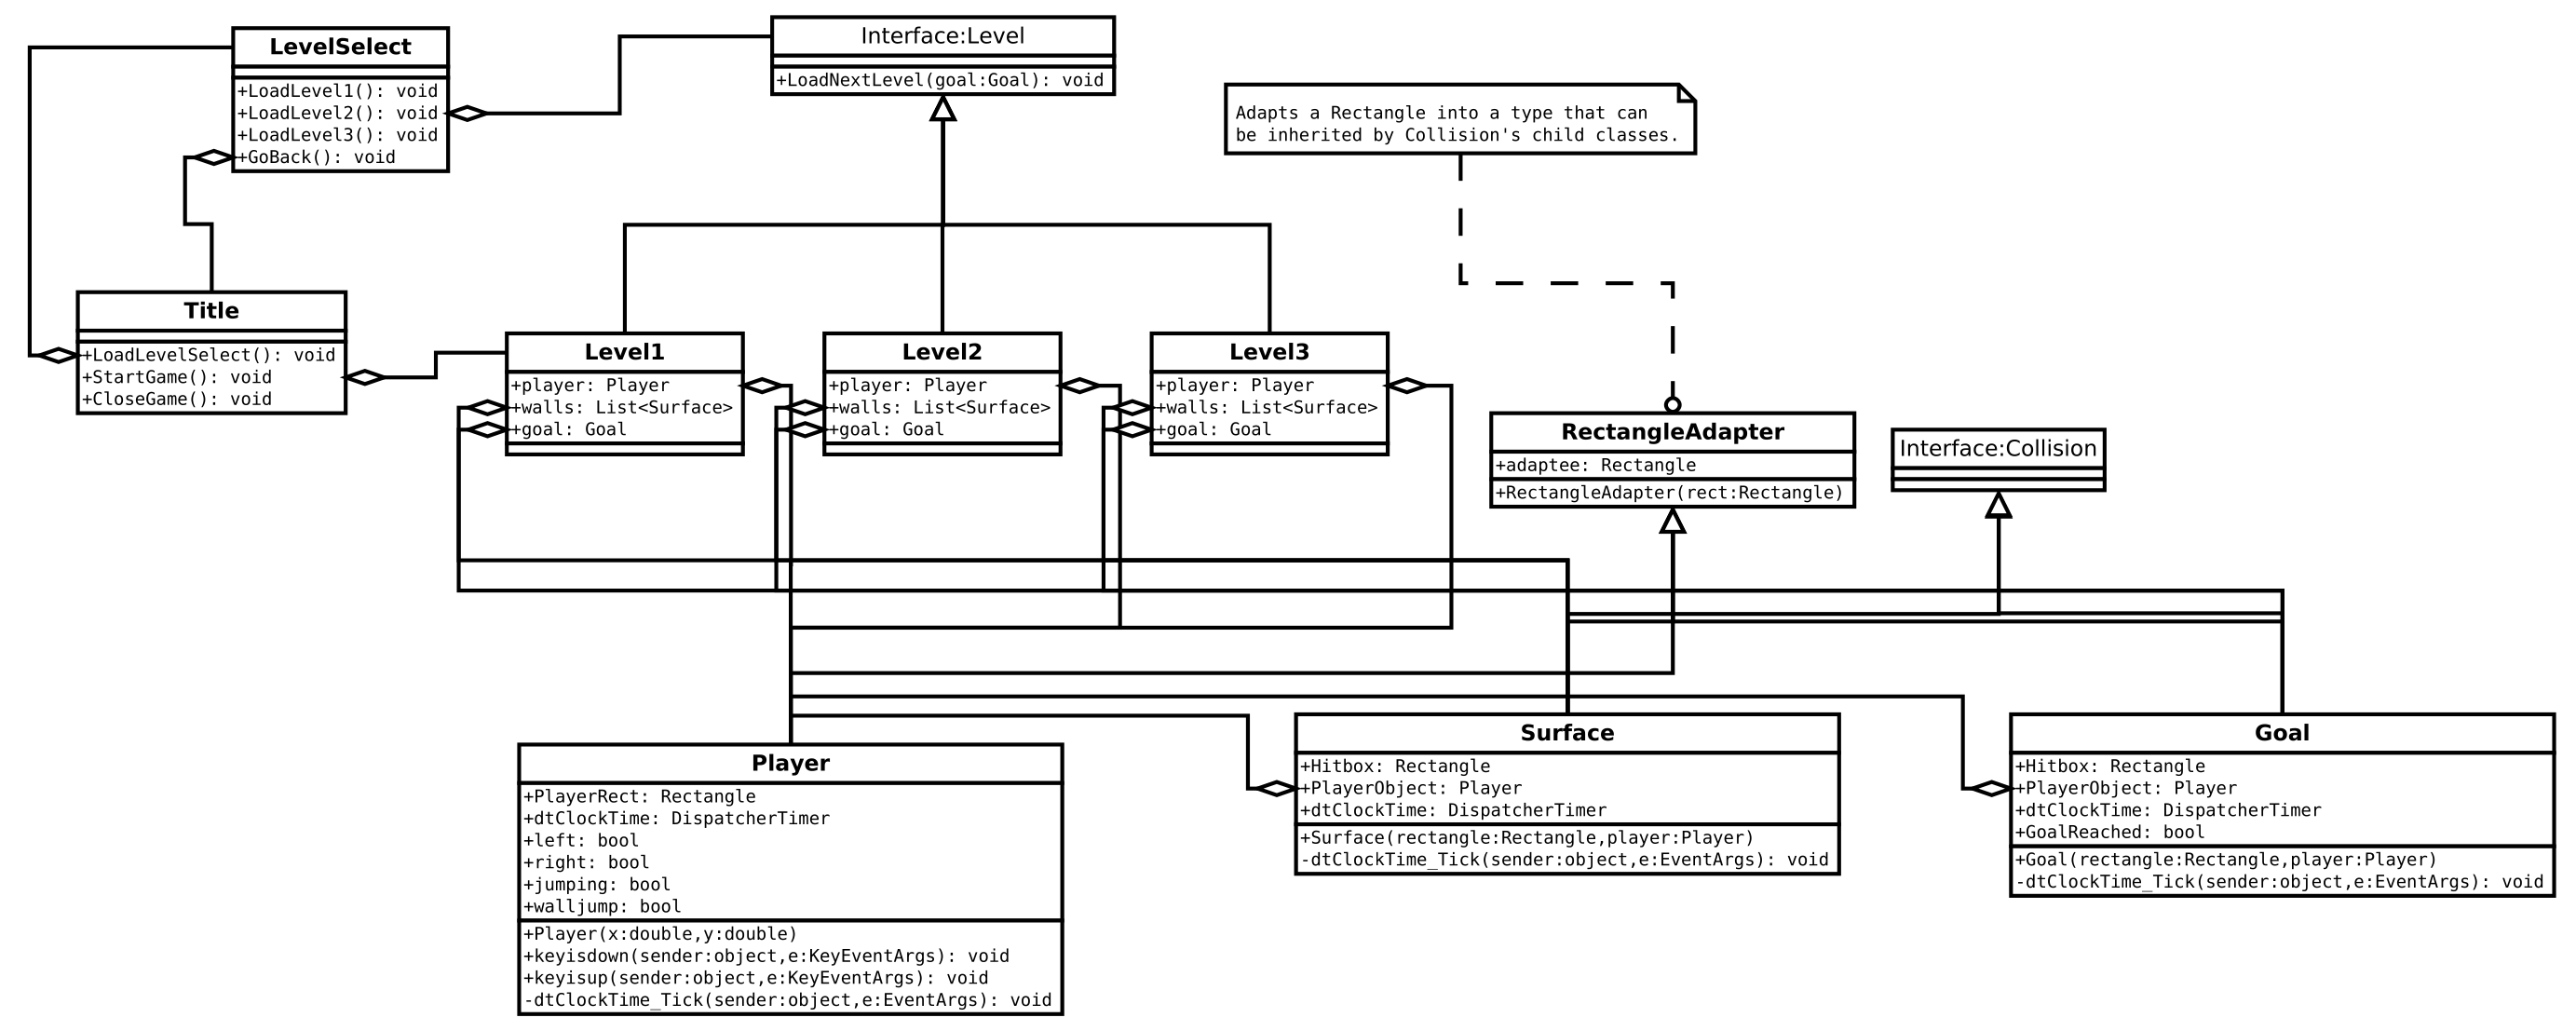
\includegraphics[height=250px, width=500px]{Penultimate_UML.png}
\caption{UML Outline}
\label{Facade}
\end{figure}

\begin{figure}[ht!]
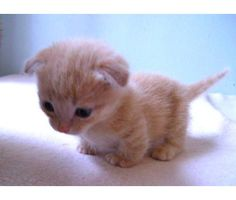
\includegraphics[scale=1.5]{cat2.jpg}
\caption{Morale Support}
\label{cat2}
\end{figure}


\subsection{Design Patterns Used}
The 2 design patterns used are the Strategy pattern and the Adapter pattern.

Strategy: On the level select, a different level is chosen depending on what button the user selects on that screen. Depending on the selection, either of 3 strategies (Levels) can be instantiated: Level1, Level2, or Level3.

Adapter: The adapter pattern is used to adapt a Rectangle into being a RectangleAdapter, which is to get around the fact that Rectangle on its own cannot be inherited from, as it is a sealed class. The Surface, Goal, and Player objects then inherit from RectangleAdapter.


\section{Results}
The project was definitely going to be hard to implement from the very moment we made the initial concept. Making a platformer in a WPF application is certainly not easy or ideal. Regardless, I'm satisfied that we managed to get something together that meets the requirements we established. The project is nearing completion, and it seems we'll have everything we wanted to include at minimum. Looking back, perhaps it wasn't the best idea to create a platformer with a WPF application.

\subsection{Future Work}
From here, we plan to potentially clean up what we have even further. After all is said and done with this project, we don't have any particular plans to do anything more with this project when it comes to distribution or anything else. We figure this will just remain as a past project.




\begin{thebibliography}{Captain Ahab}
\item Wasn't sure how to remove this.
\end{thebibliography}


\begin{IEEEbiography}{Michael Shell}
Biography text here.
\end{IEEEbiography}

% if you will not have a photo at all:
\begin{IEEEbiographynophoto}{John Doe}
Biography text here.
\end{IEEEbiographynophoto}

% insert where needed to balance the two columns on the last page with
% biographies
%\newpage

\begin{IEEEbiographynophoto}{Jane Doe}
Biography text here.
\end{IEEEbiographynophoto}





% that's all folks
\end{document}


